\documentclass[11pt, a4paper]{article}

\usepackage{graphicx}
\usepackage[english]{babel}
\usepackage[utf8x]{inputenc}
\usepackage{amsmath}
\usepackage[a4paper,top=3cm,bottom=2cm,left=2cm,right=2cm,marginparwidth=1.75cm]{geometry}
\usepackage{amssymb}
\usepackage{subfig}

\graphicspath{ {./images} }

\makeatletter
\renewcommand*\env@matrix[1][*\c@MaxMatrixCols c]{%
  \hskip -\arraycolsep
  \let\@ifnextchar\new@ifnextchar
  \array{#1}}
\makeatother

\begin{document}

\setcounter{section}{8}
\section{Lecture 9 (09/03/2020)}
\subsection{The moment of Inertia}
The moment of inertia is a mathematical desription of resistance to accelerating rotation.
This is not to be confused with the area moment of inertia\footnote{ as seen in WB1631-15 Mechanics of Materials} which is the same physical quantity and the
same integral but over an area  rather then a mass-density function. The integral describing the moment of
Inertia of a rigid body with 1 or 2 dimensions are as follows: 
\begin{gather}
  \int \rho(x)r^2\,dx\\
  \iint \rho(x, y)r^2\,dA
\end{gather}
This resistance to rotation term appears quiet naturally when analyzing a rotating body.
\begin{figure}[h]
  \centering
  \subfloat[1 mass]{{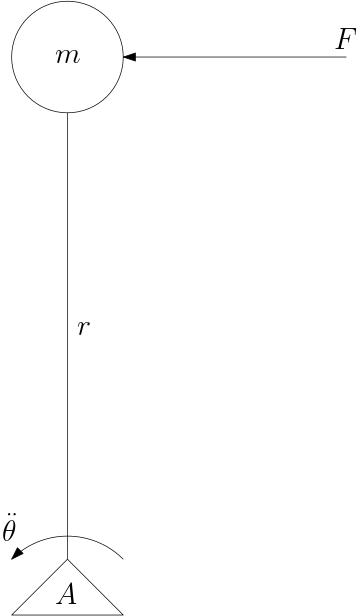
\includegraphics[width=30mm]{images/Single_mass.png}}}%
  \qquad
  \subfloat[2 masses]{{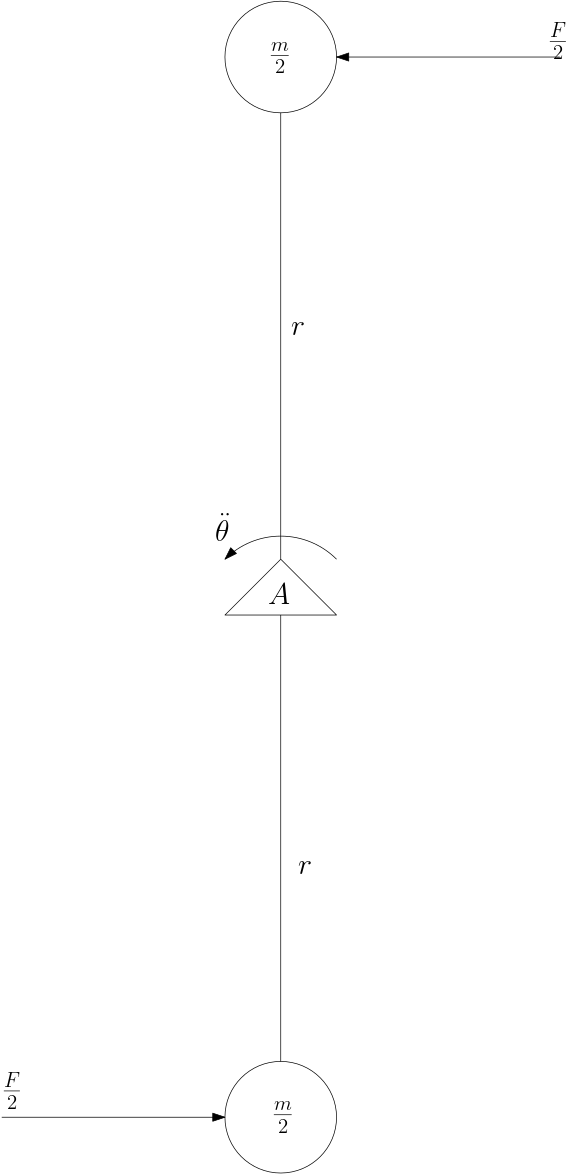
\includegraphics[width=30mm]{images/Double_mass.png}}}%
  \caption{Rigid body with mass at the end of a stick}
\end{figure}
\begin{gather}
  \Sigma r\cdot F = rma\\
  a = r\alpha = r\ddot{\theta}\\
  M_A = rF\\
  \Sigma M_A - mr^2\ddot{\theta} = I_A \ddot{\theta}
\end{gather}
Looking at Figure 1 (b) it's easy to see that it does not matter if there is a single mass with a force $F$
acting on it or 2 masses with a force $\frac{F}{2}$ acting on them. This proces of adding more and more masses
can be repeated indefenitly. This creates a circle with radius $r$. This circle is referred to as the 
radius of gyration. Only mass and radius of Gyration are needed to compute the moment of inertia.
Any given object will always want to rotate about it's center of gravity. Orientation and location
of the object in space do not matter. When an object is not attached at the center of gravity such as
figure 2 shows an extra term needs to be accounted for in the moment of inertia. This term is referred to
as the Steiner term. It takes the following form:
\begin{gather}
  \Sigma M_O = (mr^2 + md^2)\ddot{\theta}
\end{gather}
where $I_G = mr^2$ and $md^2$ the Steiner term. Note that I would add an image to visualize, but LaTeX is being a 
prick about it so you can google it or look at the book or something.\\
\\
\newpage
\underline{Moment of inertia of a 1D body:}
\begin{figure}[h!]
  \centerline{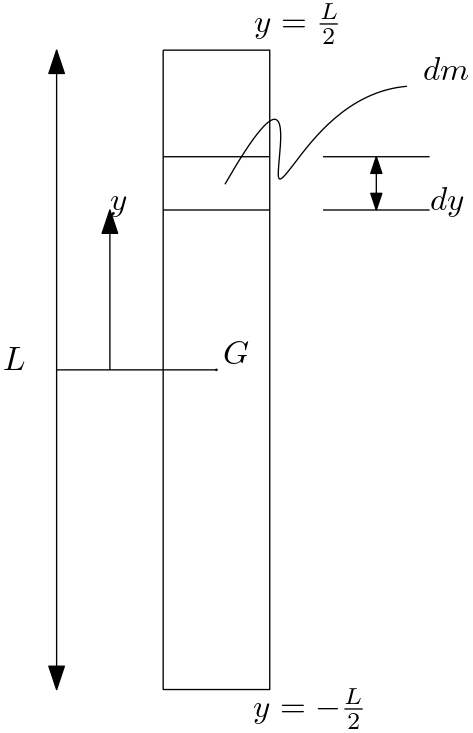
\includegraphics[width=50mm]{images/1D.png}}
  \caption{1 dimensional bar for determening the moment of inertia}
\end{figure}
\begin{gather}
  \text{Assuming the width is much less then the lenght reduces this to a 1D problem.}\notag\\
  \frac{d\rho}{dL} = 0 \Rightarrow \rho = \frac{m}{L}\\
  dm = \rho dy\\
  dI_G = ydm = \rho y^2 dy\\
  I_G = \int_{-\frac{L}{2}}^{\frac{L}{2}} \rho y^2\,dy = \frac{1}{3}\rho y^3\Big|_{-\frac{L}{2}}^{\frac{L}{2}}\\
  I_G = \frac{1}{12}\rho L^3 = \frac{1}{12}mL^2\\
  \text{When not rotating about the center of gravity:}\notag\\
  I_A = I_G + md^2\text{, where $md^2$ is the Steiner term}\\
  I_A = \frac{1}{12}mL^2 + \frac{1}{4}mL^2 = \frac{1}{3}mL^2
\end{gather}\\
\\
\underline{Moment of inertia of a 2D body:}
Might add this later

\subsection{Equations of motion}
Since we are now considering rigid bodies in a 2D space rather then just point masses we should
also consider the effects of rotation\footnote{Some people prefer to define point masses as not being able
to rotate others as define them as having no inertia, it doesn't really matter}. The new set of equations
of motions will be the following:
\begin{gather}
  \begin{cases}
    \Sigma F_x = m\ddot{x}\\
    \Sigma F_y = m\ddot{y}\\
    \Sigma M_G = I_G\ddot{\theta}
  \end{cases}
\end{gather}
It's important to note that in Statics we where free to choose any given point to calculate the moment sum,
since the entire body was in static equilibrium. This concept does NOT hold for dynamics. The center of rotation
matters and cannot be chosen freely due to the effect of Steiner terms.

\subsection{Example of a pendulum type motion as a rigid body}
\begin{figure}[h]
  \centerline{\includegraphics[width=50mm]{images/pendulum.png}}
  \caption{An object which will swing in a pendulum type motion}
\end{figure}

\begin{gather}
  \Sigma M_A = \frac{L}{2}mg\sin(\theta) = I_A\ddot{\theta}\\
  \text{This is a non-linear second order differential equation}\notag \\
  \text{To make solving this easier we assume small angles} \notag \\
  \theta << 1 \Rightarrow \sin(\theta) \approx \theta\\
  \ddot{\theta} + \frac{Lmg}{2I_A} \theta = 0\\
  r^2 +  \frac{Lmg}{2I_A} r = 0\\
  r = 0 \pm i\sqrt{\frac{Lmg}{2I_A}}\\
  \alpha = 0 \quad \beta = \omega_n = \sqrt{\frac{Lmg}{2I_A}}\\
  y_c = e^{\alpha t}(A\sin(\beta t) + B\cos(\beta t))
\end{gather}

\end{document}